If we want to understand how two states interact in international politics, we need to know how similar their foreign policy preferences are. If states have similar preferences, it is difficult to imagine how these states would come into conflict--since their is little to fight over. Conversely, if states' preferences are highly dissimilar, we would expect conflict to be more likely, and cooperative encounters to be markedly less likely. Unfortunately, while we have abundant data to measure the strength of states' economies, the volume of trade between states, or even their military power, it is much more difficult to measure states' preferences, because they are not observable.

Effectively measuring state preferences would yield scholars a number of benefits. First, foreign policy preferences are interesting in their own right--we have reason to suspect, for example, that the foreign policy preferences of the United States under President Trump have diverged from those of traditional allies like Germany and Canada, and moved in the direction of countries like Russia, Saudi Arabia and the UAE--and with an effective measure of preferences, we could better understand what causes them to change. Second, foreign policy preferences play important roles in theories on a wide range of topics including mediation, crisis bargaining, and coalition dynamics \citep{kydd:2003, gallop:2017, wolford:2014}. If we want to test these theories, we need an accurate measure of these preferences. Similarly, the democratic peace, which has been called ``the closest thing to a law in international relations" requires an accurate measure of preferences to determine whether their is something intrinsic to democracy reducing the risk of conflict \citep{oneal:russett:1999e}, or if democracies simply have more similar preferences and thus are less likely to quarrel \citep{farber:gowa:1995, gartzke:1998}. Finally, from the perspective of predicting and preventing conflict, a better measure of state preferences could help us predict where conflict is most likely to occur, and where peacebuilding resources could be best deployed.

Much of the extant literature has focused on estimating state preferences by utilizing spatial weighting models on either alliance behavior or United Nations (UN) voting scores. These approaches have proven to be useful but there are two reasons to desire a different approach. First, alliances are rare and voting together in the UN is very common, so, by only focusing on the direct dyadic behavior, we risk mischaracterizing important relationships. Second, we would expect a better understanding of state preferences to help us predict state behavior, but as we show in Figure \ref{fig:rocShitty} adding measures of state preferences to a traditional model of interstate disputes yields relatively scant increases in our predictive ability.

\begin{figure}[ht]
	\centering
	\begin{tabular}{cc}
	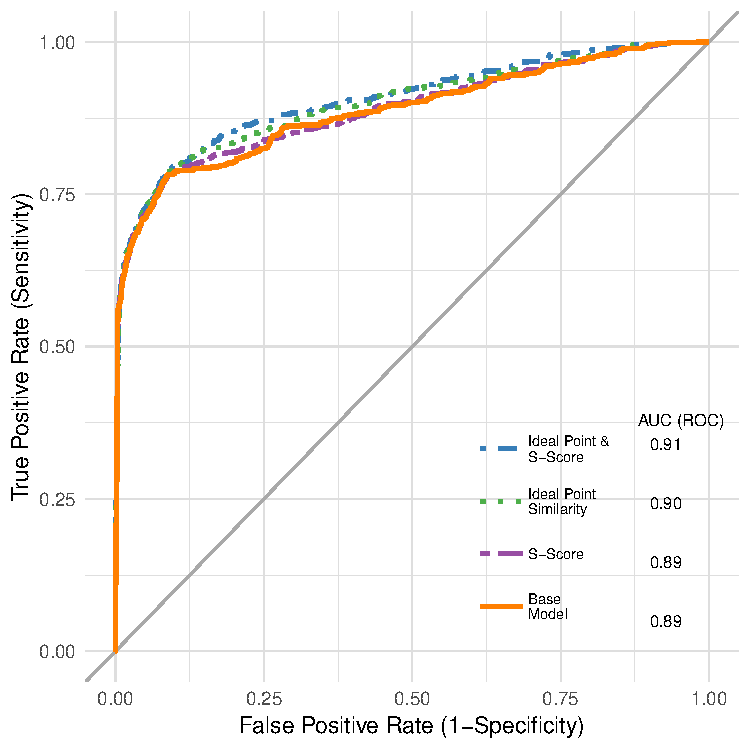
\includegraphics[width=.5\textwidth]{roc_outSample_noLatAngle.pdf} & 
	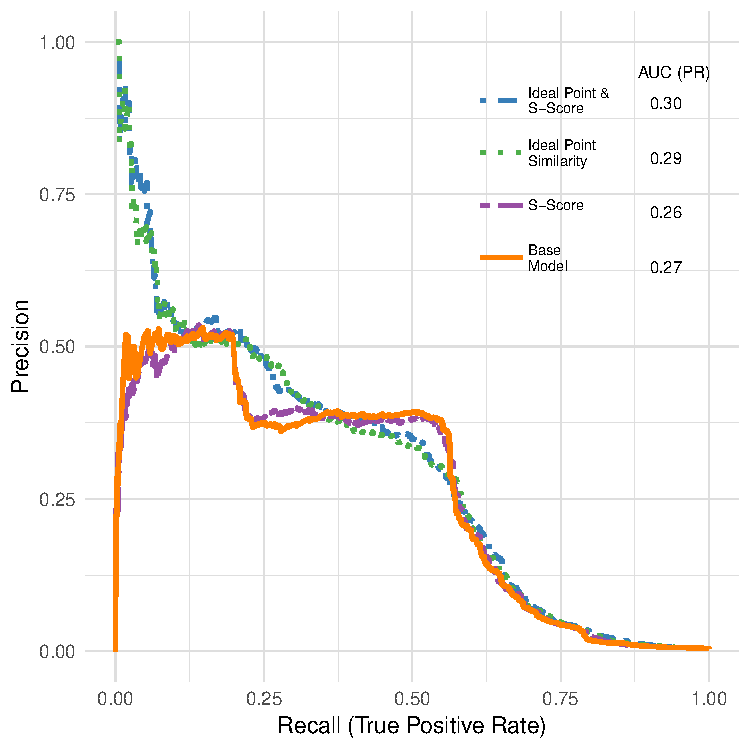
\includegraphics[width=.5\textwidth]{rocPr_outSample_noLatAngle.pdf}	
	\end{tabular}
	\caption{Assessments of out-of-sample predictive performance of Militarized Interstate Disputes using ROC curves and PR curves. AUC statistics are provided as well for both curves.}
	\label{fig:rocShitty}
\end{figure}


We can improve on these measures of preferences using the same raw material by acknowledging that both alliance membership and UN voting are layers of relationships that constitute a multilayer network, in which the various layers correspond to different ways states are interacting with one another at a given time point. A bevy of research has shown that accounting for network structure necessitates an approach that can account for the indirect relations states share. As such, we make two contributions to the existing literature on state preferences. We introduce a latent factor model that accounts for higher-order dependence patterns across multiple layers. We show that our revised approach of measuring state preferences both better characterizes relationships that have had counterintuitive results, and this measure greatly enhances our ability to predict instances of conflict.

